% !TeX root = ../../main.tex
\chapter{Implementation}
\label{chapter:scafi3-arch-reification}

This chapter discusses the instantiation of the proposed abstract architecture described in \Cref{chapter:contribution} to ScaFi3.
%
\todo{link to de luigi thesis for pure core module, that is not part of this work}

\todo{description of the flow}

\todo{high level architecture modules view}

\todo{project structure - shared, jvm-native, js-native, js, native, jvm and expect/actual Scala mechanism}

\section{High level architecture}

\section{Infrastructure module}

\subsection{Distribution module}

Enabling distribution in ScaFi3 requires implementing an abstract network manager that is able to send and receive Value Trees \todo{in context add Value Tree} from and to neighbor devices.
%
The AC framework abstract over the specific protocol used to communicate and the neighborhood discovery mechanism, allowing the implementation of different network managers for different protocols and scenarios.

As a first step towards a full-featured distributed ScaFi3, a socket-based network manager has been implemented, leveraging stream, TCP-based connection-oriented sockets.
%
As shown in \Cref{fig:socket-network-manager-architecture}, each device is bound to a specific endpoint (IP address and port) and communicates point-to-point with its neighbors.
%
\begin{figure}
    \centering
    \includegraphics[width=\textwidth]{resources/img/socket-network-manager.pdf}
    \caption{Socket-based network manager high level architecture.}
    \label{fig:socket-network-manager-architecture}
\end{figure}

Despite the low-level nature of sockets, they provide a foundational abstraction layer that many higher-level protocols ultimately rely upon (such as HTTP, MQTT, etc.), making them a suitable starting point for building extensible communication mechanisms.

\begin{figure}
    \centering
    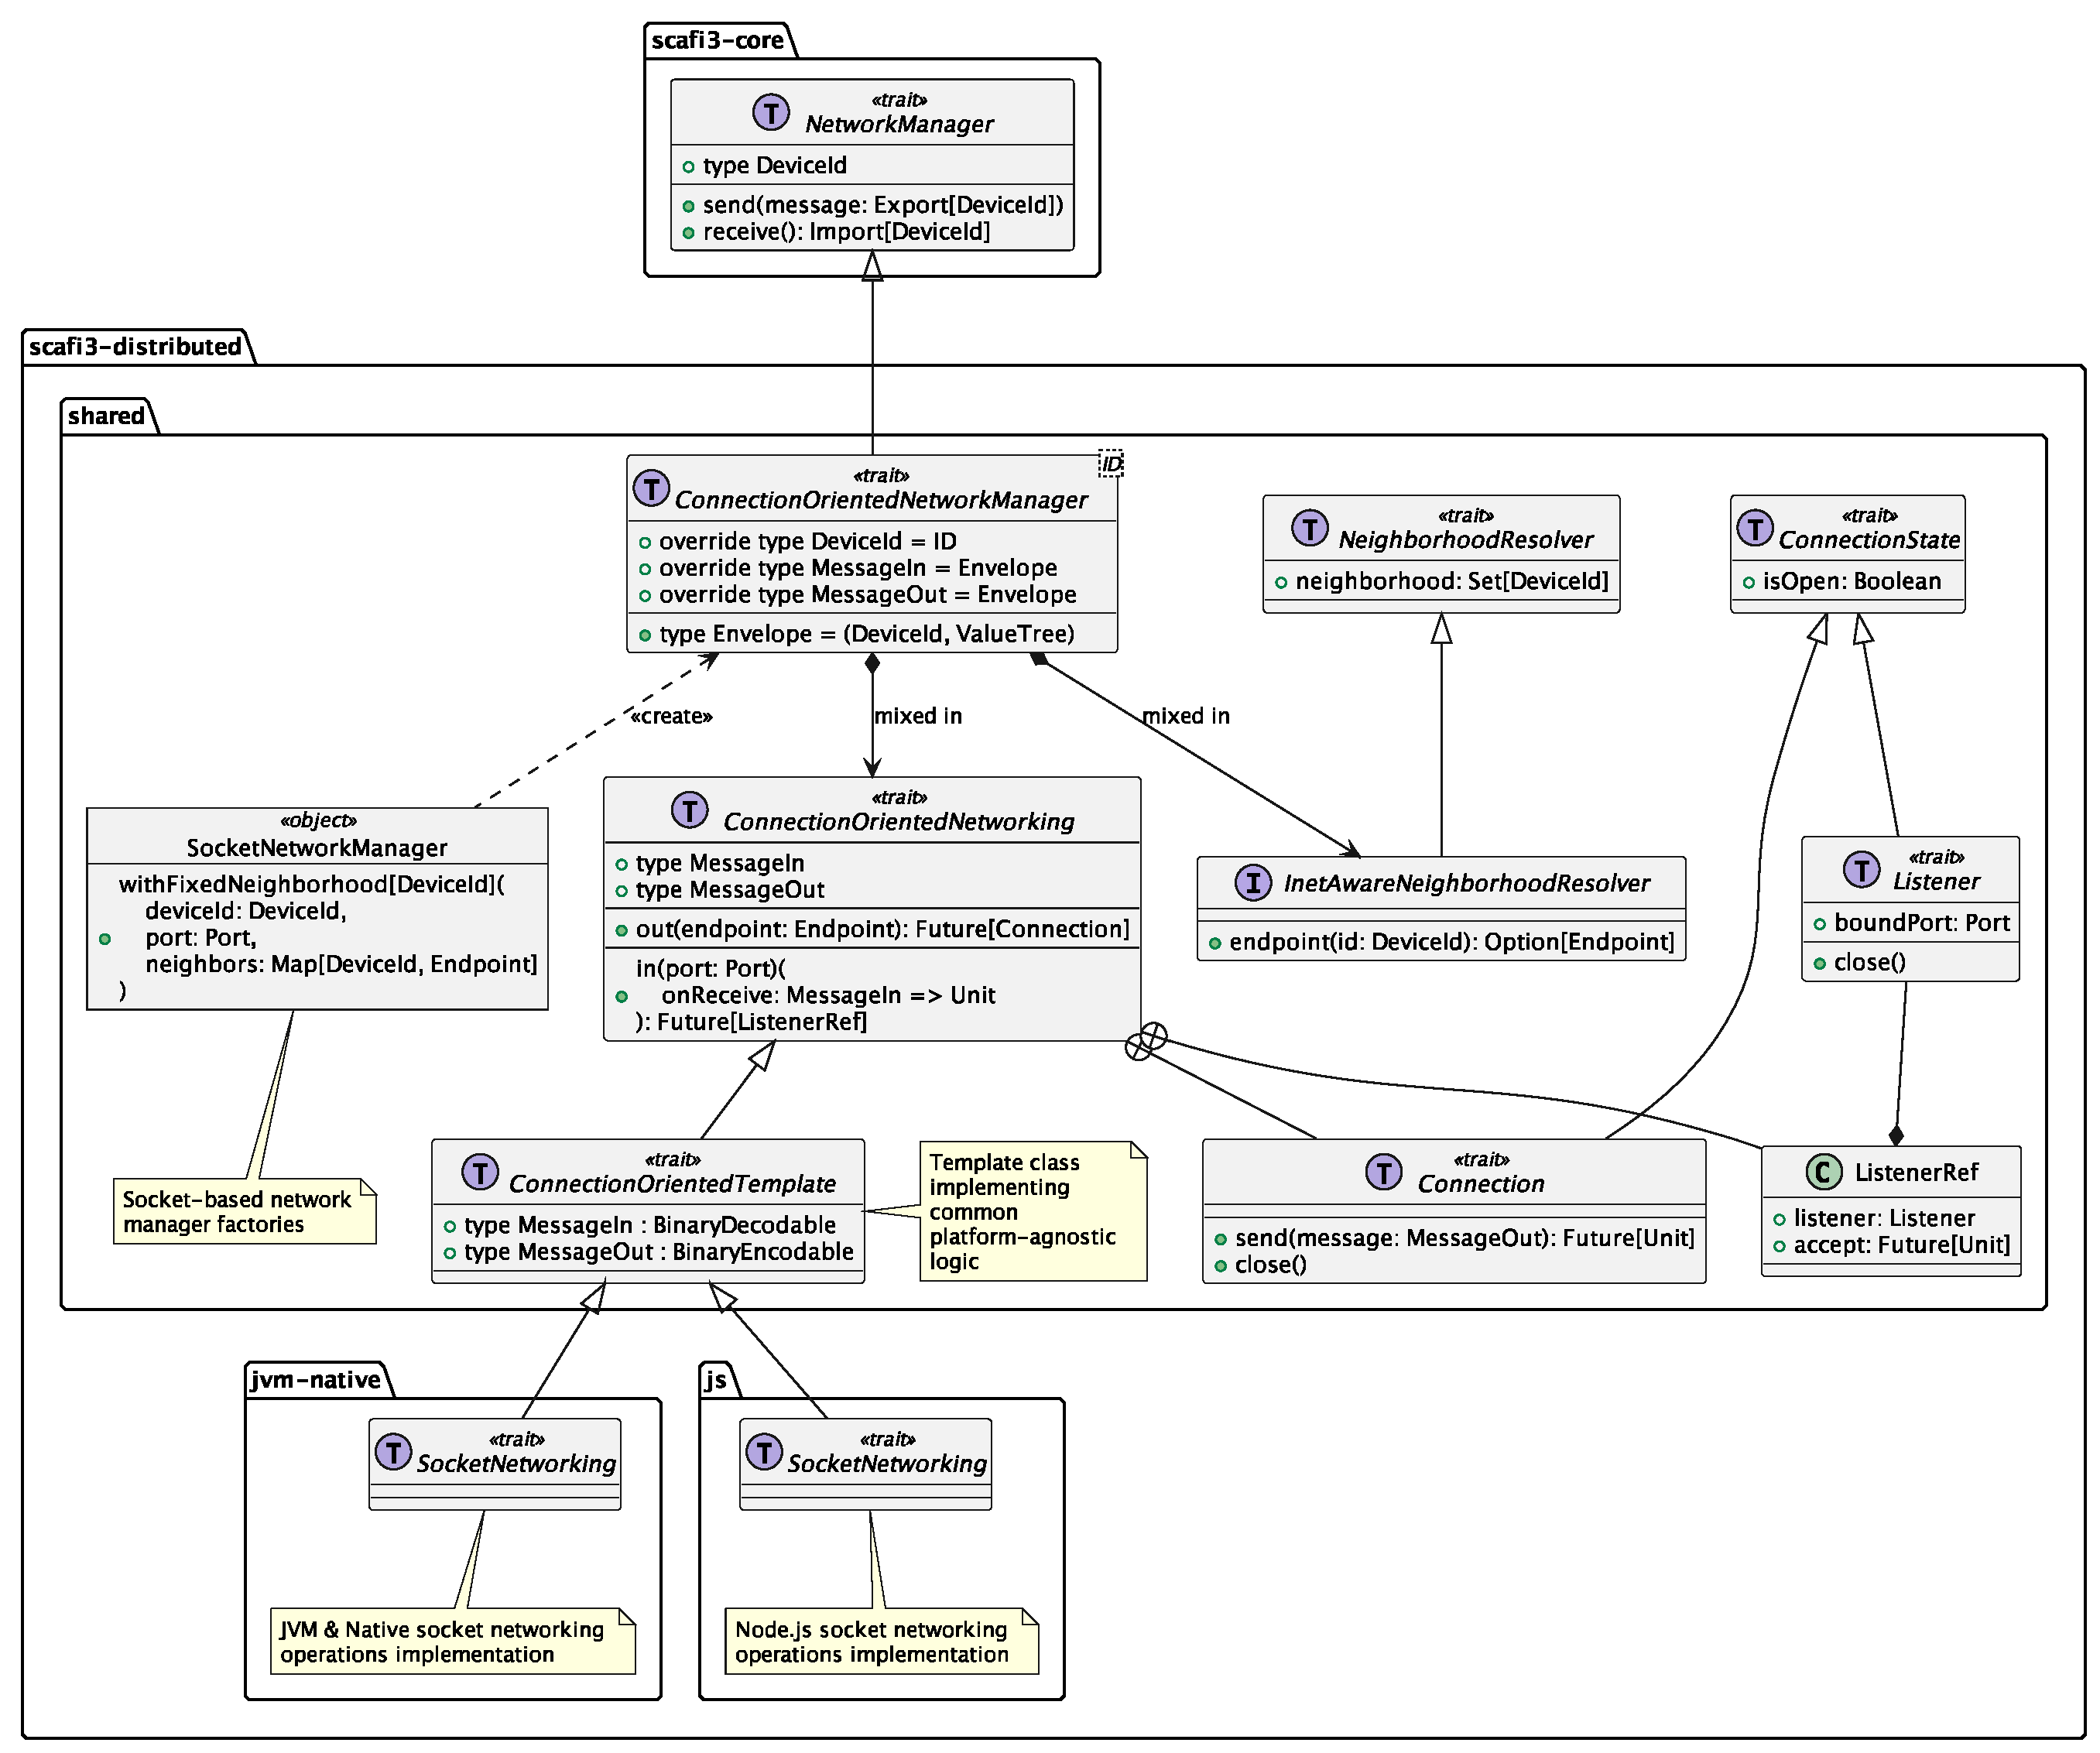
\includegraphics[width=\textwidth]{resources/schemas/socket-distribution.eps}
    \caption{UML diagram of the socket-based network manager design.}
    \label{fig:socket-network-manager-design}
\end{figure}






% \subsection{Protobuf serialization binding}

% \subsection{Platform-specific library abstraction layers}

% \section{Implementation challenges and solutions}
